\documentclass[12pt,oneside,a4paper]{report}
\usepackage{mathtools}
\usepackage[HTML, hyperref, svgnames, table]{xcolor}
\usepackage[utf8]{inputenc}
\usepackage{polski}
\usepackage[polish]{babel}
\usepackage{multicol}
\usepackage{graphicx} 
\usepackage[margin=1in]{geometry}

\begin{document}
\begin{titlepage}
   \begin{center}
        \vspace*{2cm}

        \large Politechnika Wrocławska Wydział Elektroniki Kierunek Teleinformatyki
        \vspace*{2cm}

        \large Inżynierska praca dyplomowa

        \vspace*{0.5cm}
        \huge\textbf{Projekt sztucznej inteligencji}

        \vspace{0.5cm}
        \normalsize 
            
        \textbf{Michał Żarejko}
        \vspace{3cm}

   \end{center}

        \setlength{\columnsep}{-20pt}
        \begin{multicols}{2}
           Dyplomant:  

           \vspace{0.2cm}
           Nr albumu:

           \vspace{0.2cm}
           Promotor:

        \columnbreak
           \textbf{Michał Żarejko}

           \vspace{0.2cm}
            \textbf{249374}

           \vspace{0.2cm}
            \textbf{dr inż. Paweł Zyblewski}
        \end{multicols}

        \vspace{0.5cm}


        \vspace{2cm}
   \begin{center}
        Wrocław. 2021


   \end{center}
\end{titlepage}


\newgeometry{top=2.5cm,bottom=2.5cm,right=2.5cm,left=3.5cm}
\tableofcontents{}
\newpage

\setlength{\parindent}{1.5em}
\setlength{\parskip}{1em}
\renewcommand{\baselinestretch}{2.0}

\chapter{Wstęp}

Duży rozwój nauki w ostatnich latach związany z uczeniem maszynowym, spowodował powstanie wielu
nowoczesnych algorytmów i technologi, które pomagają dzisiaj w codziennych czynnościach lub 
zastępują ludzi w odpowiedzialnych procesach. 

Przykładem mocno rozwijanych narzędzi używanych w życiu
prywatnym są asystenci głosowi, tłumacze maszynowe, modele wyświetlające elementy na
stronach internetowych na podstawie gustu użytkownika, gry wideo, inteligentne samochody lub przetwarzanie 
obrazów. Dodatkowo uczenie maszynowe jest mocno wykorzystywane w większości firmach, między 
innymi na halach produkcyjnych, w transporcie, medycynie, cyberbezpieczeństwie. 

Po mimo tak wielu możliwości i zastosowań, sztuczna inteligencja zyskuje największą popularność
medialną przez gry rywalizacyjne, gdzie głównym zadaniem jest pokazanie przewagi algorytmów względem
ludzi. W ostatnich 20 latach można spotkać się z dużą ilością wydarzeń gdzie profesjonalni gracze 
muszą stoczyć pojedynek z wytrenowaną sztuczną inteligencją. Między innymi w 2016 roku zorganizowano
mecz między 18 mistrzami świata w grze "Go", mieli oni za zadanie pokonać algorytm "AlphaGo"
utworzony przez zespół "DeepMind". Dużym osiągnięciem była wygrana modelu z wszystkimi
graczami, gra była uważana powszechnie za skomplikowaną i trudną do rozwiązania.

W 2019 roku zespół "OpenAI" utworzył grupę współpracujących "botów" w grze komputerowej
"Dota 2". W 4 dniowym wydarzeniu odbywającym się internetowo modele rwalizowały z 5 osobowymi
grupami. Maszyny AI zdołały pokonać dużą część graczy. Wydarzenie było mocno omawiane z powodu
poziomu skomplikowania gry. Dla porównania środowisko  gry "Go" zawiera 150 możliwych ruchów na turę, "Dota 2"
może posiadać ich 20 000 przez czas 45 minut.

Takie wydarzenia pokazały, że w dzisejszych czasach sztuczna inteligencja może przewyrzszać
myśleniem strategicznym człowieka.
Często w tworzeniu takich programów dużym wyzwaniem jest poziom skomplikowania gry, 
zależy to między innymi to od tego, czy jest to środowisko deterministyczne, czy stochastyczne, 
czy głównym zadaniem jest rywalizacja czy, współpraca, ile modeli ma zawierać gra.
Aktualnie jednak jednym z największych problemów takich programów jest niedostateczny
zakres dostępnych informacji o środowisku. Sztuczna inteligencja, aby zwyciężać
musi zostać nauczona grać, więc potrzebuje dużej ilości danych wejściowych, które są 
rozróżnialne. Przykładem gry, która jest pozbawiona tego problemu są szachy. 
Sztuczna inteligencja wykonuje ruchy bazując na informacjach w jaki sposób są ułożone pionki
w danym momencie i na historii dotychczasowej gry. Zmiana stanu środowiska jest
zauważalna przez gracza co pozwala na natychmiastową reakcję i prostsze sposoby na uczenie
maszynowe. Przykładem gry ciężkiej do rozwiązania, w której występuje nie pełny zestaw informacji 
jest Poker Texas Holdem, po mimo wiedzy o kartach w ręce i na stole, gracz nie posiada wiedzy o 
kartach przeciwników, w takim przypadku dwa pozornie identyczne stany środowiska w
rzeczywistości mogą się różnić. Z powodu takich cech większość popularnych algorytmów jak 
"DQN", "Actor-Critic" lub "AlphaZero" staje sie bezużyteczna i nie daje dobrych rezultatów.

W niniejszej pracy przedstawiono sposób możliwego rozwiązania takiego problemu przy pomocy 
algorytmu o nazwie "Deep CFR". Pierwszy i drugi rozdział dokładnie opisuje cele pracy, zakres projektu, 
zagadnienia wymagane aby zrozumieć działanie algorytmu. W trzecim rozdziale skupiono się na
implementacji, czwarty pokazuje uzyskane wyniki.


\section{Cel i zakres pracy}

Głównym celem pracy jest implementacji algorytmu "Deep CFR" do gry "Heads Up Limit Texas 
Poker Hold'em". Jest to popólarna wersja rozgrywki 2-osobowej gdzie uczestnicy nie mogą wybrać
samodzielnie kwoty podbicia stawki, jest ona ograniczona przez ustaloną wartość. Takie środowisko
minimalizuje możliwe ruchy do 3 akcji. Używając omawianego algorytmu
wytrenowano 5 modeli rozpoznawania, które zostały następnie wykorzystane do rozegrania
turnieju składającego się na wszystkie kombinacje rozgrywek modeli po
10 powtórzen gry. Taki proces pozwoli określić, który model najlepiej gra w 
"Heads Up Limit Texas Poker Hold'em". 

\section{Przegląd dostępnych rozwiązań}

W ciągu ostatnich 10 lat powstało wiele algorytmów rozwiązujących różne werjse gry Poker.
Miedzy innymi "Extensive-Form Fictitious Play", "Neural Fictitious Self-Play",
"Regret Policy Gradients", "Counterfactual Regret Minimization". 
Z wymienionych algorytmów popólarnym aktualnie rozwiązaniem jest "CFR" rozszerzony o sieci neuronowe,
zwany "Deep CFR". Daje on najszyszą zbierzność \cite{dcfr}.

\subsection{Teoria Gier}

Aby zrozumieć działanie wymienionych algorytmów nalerzy zapoznać się
działem matematyki o nazwie "Teoria Gier" \cite{gt}. Bada on optymalne zachowanie w grach
hazardowych przez dobieranie odpowiedniej strategii bazującej na zasadzie "Równości Nasha" oraz 
opisie środowiska jako gry w postaci ektensywnej.

\subsubsection{Gra w postaci ekstensywnej}

Aby rozwiązać skąplikowane grę należy ją przeanalizować przy pomocy uproszczonego opisu. Gry w
formie ekstensywnej można przedstawić jako drzewo decyzyjne gdzie każdy węzeł rozgałęzia się na
możliwe akcje oraz identyfikuje aktualny stan gracza przez zestaw informacji I,
ostatnie węzły to stany końcowe gdzie określony gracz zyskuje nagrode lub ją traci.
Poniewż drzewo przedstawia grę wielu graczy, dlatego każdy z węzłów należy przypisać odpowiedniemu
uczestnikowi. 

\begin{figure}[h!]
  \centering
  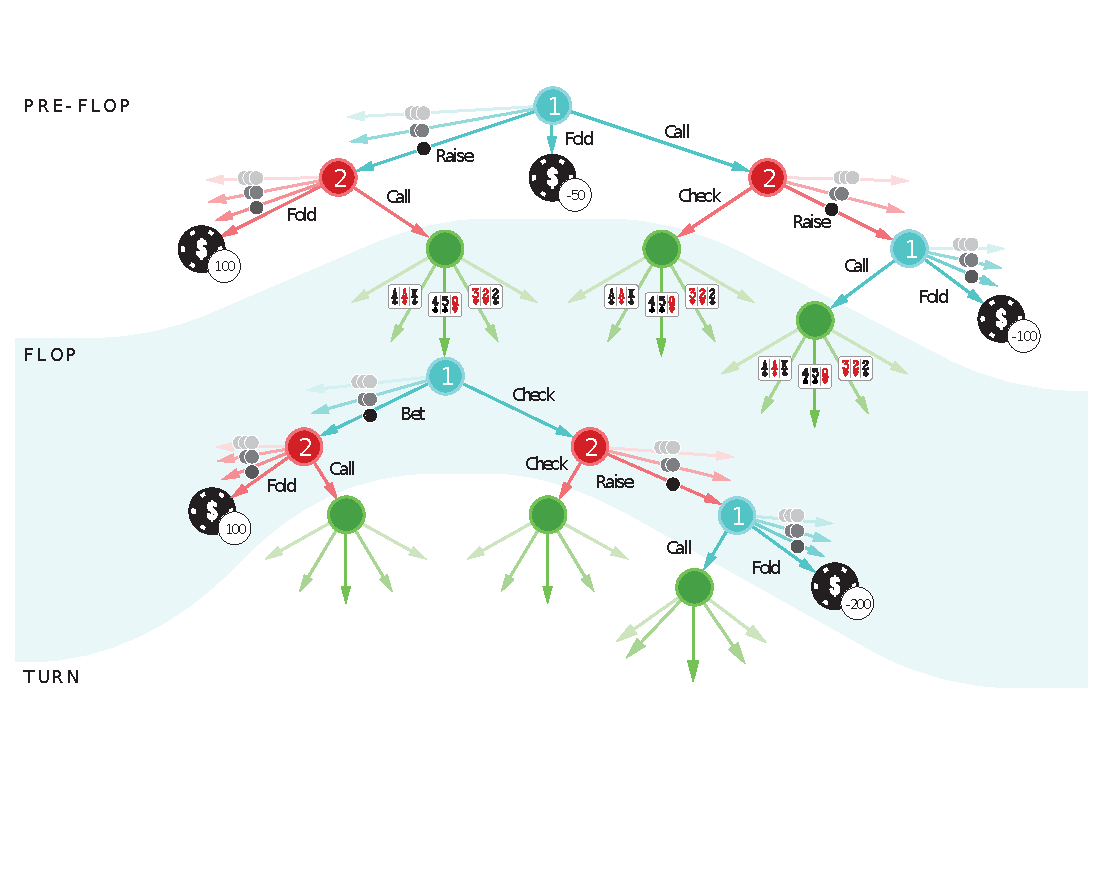
\includegraphics[width=0.7\textwidth]{./img/tree1.pdf}
  \caption{Drzewo decyzyjne gry "No-limit Poker Texas Hold'em". \cite{ds}}
\end{figure}


\subsubsection{Równość Nasha}

W grach postaci normalnej \cite{n} to twierdzenie określa perfekcyjny stan gry gdzie wszyscy gracze wykorzystują najlepszy
zestaw strategii, którego zmiana przyniesie tylko straty. Oznacza to, że nie jest możliwe
zwiększenie uzyskanej nagrody bedąc w tym stanie \cite{gt}.

\subsubsection{Podział gier}

Dodatkowo dział nauki zakłada, że omawiane środowiska można podzielić na gry o sumie stałej, 
zmiennej oraz zerowej. Wszystkie wymienione formy opisują różnice między wygraną i przegraną 
graczy. W pracy założono, że "Heads Up Poker Texas Hold'em" jest grą
2-osobową o sumie zerowej, czyli wygrana jednego
uczestnika oznacza całkowitą porażkę oponenta w wyskokości wygranej stawki w taki sposób, że suma 
wygranej i przegranej wynosi zero. W takiej formie można
zaimplementować "Deep CFR", który ma szanse zbiec się do stanu bliskiego "Równości Nasha" \cite{dcfr}.
Algorytm będzie przez wiele iteracji eksplorował drzewo decyzyjne i dobierał odpowiednie 
strategie aż trafi na takie, które dają najlepsze rezultaty.

\subsubsection{Metryki}

Popólarnym sposobem badania postępów modelu względem bliskości Równości Nasha jest metryka "Exploitabilit"
czyli różnica między najlepszą możliwą strategią w grze, a aktualnym modelem.

\subsection{Historia modeli Poker Texas Hold'em}

Bazując na teorii gier oraz różnych algorytmach powstało wiele rozwiązań różnych wersji gry Poker.
Pierwsze dokumenty naukowe badające grę zaczęły powstawać w 2005 roku omawiające bardzo proste
środowiska jak "Poker Kuhn", na pierwszy duży sukces trzeba było czekać 10 lat.
W 2015 roku utworzono sztuczną inteligencje "Cepheus" rozwiązującą problem
"Heads Up Limit Texas Hold'em" wykorzystujące algorytm CFR+. Po tym osiągnięciu rozpoczęto prace nad
algorytmem mogącym rozwiązać problem gry "Heads Up No-limit Texas Hold'em". Zajeło to 2 lata od 
"Cepheus'a", model nazwano "DeepStack", mieszał on techniki znane z CFR z siecimi neuronowymi. 
Przetestowano go na 33 profesjonalnych graczach w wielu iteracjach gry. Algorytm w większości
przypadków wygrał \cite{ds}. Była to pierwsza wygrana AI z człowiekiem w najtrudniejszej wersji gry Poker.

\chapter{CFR}

\section{Regret Matching}

Jest to metoda uczenia polegająca na minimalizacji żalu używana w algorytmie CFR.
Opisuje się to jako sposób na liczenie wektorów wag o długości równej liczbie możliwych akcji A
, korztstając z $u^{t}$ czyli nagrody uzyskanej w stani t oraz z dystrybucji ruchów $p^{t}$ \cite{rmg}. 
Posiadając te informacje algorytm iteracyjnie aktualizuje wagi wzorem 2.1.


\begin{equation}
p^{t}_{i}\left( a \right) = \left\{ \begin{array}{ll}
      \frac{R^{t-1, \text{+}}\left(a\right)}{ \Sigma_{a' \in A} R^{t-1,\text{+}}\left(a'\right)} &
      \mbox{if $\Sigma_{a' \in A} R^{t-1,\text{+}}\left(a'\right) >
      0$};\\
      \frac{1}{|A|} & \mbox{$otherwise$}.\end{array} \right. \ 
\end{equation}

Gdzie $R^{t} \text{(a)}$ jest równe formule 2.2, a $R^{t,\text{+}}(a)$ oblicza się jak w 2.3.

\begin{equation}
   R^{t} (a) = \frac{1}{T} {\sum_{t=1}^{T} u^{t} (a)} - \sum_{a \in A} p^{t} (a) u^{t} (a)
\end{equation}

\begin{equation}
   R^{t,\text{+}}(a) = max(R^t(a),0)
\end{equation}

Podsómowując pwyżesze wzory, dla każdej akcji wektora w danym stanie wylicza się $R^{t}(a)$, gdzie
należy skorzystać z sumy przyszłych wartości $u^{t}(a)$ oraz $p^{t}(a)$ 
dla wybrania danych ruchów. Całość obrazuje jak bardzo gracz żałuje wybranych
akcji w czasie od t do T.

\section{Regret Minimization}

W przypadku algorytmu CFR i gry Heads Up Limit Texas Hold'em gracz ma do zynienia z wyborem strategi
$\sigma_{i}^{t}$ dlatego wylicza się wartość zwaną 'Average overall regret', która określa jak gracz
i będzie żałował wybór danej strategi aż do czasu T \cite{rmg}.

\begin{equation}
   R^{T}_{i} = \frac{1}{T} \max_{\sigma^{*}_{i} \in \Sigma_{i}} \sum_{t=1}^{T}
   \left(u_{i}\left(\sigma_{i}^{*}, \sigma_{-i}^{t}\right) - u_{i}(\sigma^{t})\right)
\end{equation}

Głównym zadaniem algorytmu CFR jest minimalizacja tej wartości dla wszystkich graczy.
Dodatkowo dla każdego gracza oblicza się średnią strategię dla 
każdego stanu I oraz akcji A \cite{rmg}.

\begin{equation}
   \sigma^{-t}_{i} \left(I\right) \left(a\right) = \frac{\sum^{T}_{t=1} \pi^{\sigma^{t}}_{i}
   (I)\sigma^{t}(I)(a)}{\sum^{T}_{t=1} \pi^{\sigma^{t}}_{i}(I)}
\end{equation}

Jesli wszyscy gracze będą dążyć do minimalizacji wartości 'Average overall regret', wtedy gra
powinna osiągnąć po wielu iteracjach stan bliski Równości Nasha \cite{rmg}.



\section{Counterfactual Regret}

\section{Monte Counterfactual Regret Minimization}
 

\begin{thebibliography}{100}
   \bibitem{gt} Myerson, Roger B. Game theory. Harvard university press, 2013.
   \bibitem{rmg} Zinkevich, Martin, et al. "Regret minimization in games with incomplete information." Advances in neural information processing systems 20 (2007): 1729-1736.
   \bibitem{dcfr} Brown, Noam, et al. "Deep counterfactual regret minimization." International conference on machine learning. PMLR, 2019. 
   \bibitem{ds} Moravčík, Matej, et al. "Deepstack: Expert-level artificial intelligence in heads-up no-limit poker." Science 356.6337 (2017): 508-513. 
   \bibitem{ss} Davis, Trevor, Neil Burch, and Michael Bowling. "Using response functions to measure strategy strength." Twenty-Eighth AAAI Conference on Artificial Intelligence. 2014. 
   \bibitem{n} Heinrich, Johannes, Marc Lanctot, and David Silver. "Fictitious self-play in extensive-form games." International conference on machine learning. PMLR, 2015. 
\end{thebibliography}



\end{document}

